\documentclass[tikz, margin=1cm]{standalone}
\usepackage{tikz, helvet, pagecolor}
\usetikzlibrary{positioning, shapes.misc}

\definecolor{red}{RGB}{230,0,0}
\definecolor{anthracite}{RGB}{51,57,65}
\definecolor{lightgray}{RGB}{239,239,240}
\definecolor{green}{RGB}{117,163,0}

\renewcommand{\familydefault}{\sfdefault}

\begin{document}
\pagecolor{lightgray}
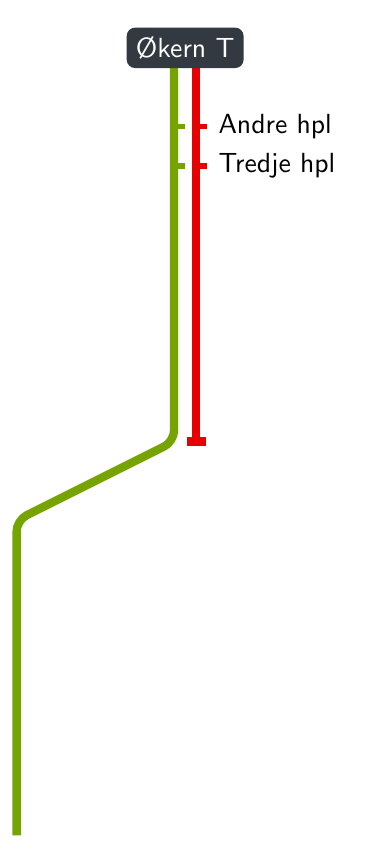
\begin{tikzpicture}[
    stop_red/.style={rectangle,
        fill=red, 
        minimum height=2pt,
        minimum width=4pt,
        inner sep=0pt,
        },
    stop_green/.style={rectangle,
        fill=green, 
        minimum height=2pt,
        minimum width=4pt,
        inner sep=0pt,
        },
    start/.style={rounded rectangle, 
        fill=anthracite, 
        text=white, 
        minimum size=4pt,
        rounded corners=3pt,
        rounded rectangle west arc=none,
        rounded rectangle east arc=none
        },
    end_green/.style={rectangle, 
        fill=green, 
        minimum height=3pt,
        minimum width=7pt,
        inner sep=0pt,
        },
    end_red/.style={rectangle, 
        fill=red, 
        minimum height=3pt,
        minimum width=7pt,
        inner sep=0pt,
        },
    ]
    \draw[line width=3pt, color=green, rounded corners, transform canvas={xshift=-4pt}] 
        (0,0) -- (0,-5) -- 
        (-2,-6) -- (-2, -10);
    \draw[line width=3pt, color=red, transform canvas={xshift=4pt}] (0,0) -- (0,-5);
    \node[start] (n_start) at (0,0) {Økern T};
    \node[end_red, transform canvas={xshift=2pt}] (l2_end) at (0,-5) {};

    \node[label={[label distance=5pt]right:{Andre hpl}}] (n2_main) at (0,-1) {};
    \node[stop_green, transform canvas={xshift=-1pt}] (n2_1) at (0,-1) {};
    \node[stop_red, transform canvas={xshift=3pt}] (n2_2) at (0,-1) {};

    \node[label={[label distance=5pt]right:{Tredje hpl}}] (n3_main) at (0,-1.5) {};
    \node[stop_green, transform canvas={xshift=-1pt}] (n3_1) at (0,-1.5) {};
    \node[stop_red, transform canvas={xshift=3pt}] (n3_2) at (0,-1.5) {};


\end{tikzpicture}
\end{document}
